\newcommand{\fileInfectorTagResultsAucTable}{
    \begin{table}[H]
        \centering
        \begin{tabular}{|p{2,8cm}||P{2,4cm} P{2,4cm} P{2,4cm}|}
            \hline
            File-infector Tag & ALOHA\newline (M/B only) & ALOHA & Proposed\newline Model \\
            \hline
            AUC-ROC & - & 0.985$\pm$0.000 & \textBF{0.987$\pm$0.000} \\
            \hline
        \end{tabular}
        \caption[File-infector Tag prediction task AUC-ROC results]{AUC-ROC (Area Under Curve) of the different models for the \textbf{File-infector Tag} prediction task. Results were aggregated over \textBF{2} training runs with different weight initializations and minibatch orderings. Best results are shown in \textbf{bold}.} \label{tab:fileInfectorTag_auc}
    \end{table}
}

\newcommand{\fileInfectorTagResultsAtFprTable}{
    \begin{center}
        \begin{longtable}[c]{|P{3,2cm}||P{1,8cm} P{1,8cm} P{1,8cm} P{1,8cm} P{1,8cm}|}
            \hline
            File-infector Tag & \multicolumn{5}{c|}{{FPR}} \\
            & $10^{-5}$ & $10^{-4}$ & $10^{-3}$ & $10^{-2}$ & $10^{-1}$ \\
            \hline
            \endfirsthead

            \caption*{\raggedright ...continued from previous page} \\
            \hline
            File-infector Tag & \multicolumn{5}{c|}{\textbf{FPR}} \\
            & $10^{-5}$ & $10^{-4}$ & $10^{-3}$ & $10^{-2}$ & $10^{-1}$ \\
            \hline
            \endhead

            \caption*{\raggedleft ...continued on next page} \\
            \endfoot

            \caption[File-infector Tag prediction task results]{Mean and standard deviation results (TPR, Accuracy, Recall, Precision and F1-Score) of the different models for the \textbf{File-infector Tag} prediction task at different \textbf{FPR}s (\textit{False Positive Rates}). Results were aggregated over \textBF{2} training runs with different weight initializations and minibatch orderings. Best results are shown in \textbf{bold}. Under \textbf{TPR} results are also presented the percentage reduction in mean detection error and in ROC curve standard deviation introduced by the \textit{Proposed Model} with respect to both \textit{ALOHA} model and \textit{Joint Embedding}.} \label{tab:fileInfectorTag_results_at_fpr} \\
            \endlastfoot

            \multicolumn{6}{|c|}{\textbf{TPR}} \\
            \hline
            ALOHA (M/B only) & - & - & - & - & - \\
            ALOHA & \textBF{0.445$\pm$0.236} & \textBF{0.520$\pm$0.206} & 0.724$\pm$0.065 & 0.844$\pm$0.001 & 0.946$\pm$0.006 \\
            Proposed Model & 0.144$\pm$0.027 & 0.326$\pm$0.047 & 0.647$\pm$0.061 & 0.854$\pm$0.003 & 0.955$\pm$0.006 \\
            \hline
            Error Reduction wrt\newline ALOHA (M/B only) & - & - & - & - & - \\
            Error Reduction wrt\newline ALOHA & -54.2\% & -40.4\% & -27.9\% & 6.4\% & 16.7\% \\
            \hline
            Std Reduction wrt\newline ALOHA (M/B only) & - & - & - & - & - \\
            Std Reduction wrt\newline ALOHA & 88.6\% & 77.2\% & 6.2\% & -200.0\% & 0.0\% \\
            \hline
            \multicolumn{6}{|c|}{\textbf{Accuracy}} \\
            \hline
            ALOHA (M/B only) & - & - & - & - & - \\
            ALOHA & \textBF{0.910$\pm$0.038} & \textBF{0.922$\pm$0.033} & 0.955$\pm$0.010 & 0.966$\pm$0.000 & 0.907$\pm$0.001 \\
            Proposed Model & 0.862$\pm$0.004 & 0.891$\pm$0.008 & 0.942$\pm$0.010 & 0.968$\pm$0.000 & \textBF{0.909$\pm$0.001} \\
            \hline
            \multicolumn{6}{|c|}{\textbf{Recall}} \\
            \hline
            ALOHA (M/B only) & - & - & - & - & - \\
            ALOHA & \textBF{0.445$\pm$0.236} & \textBF{0.520$\pm$0.206} & 0.724$\pm$0.065 & 0.844$\pm$0.001 & 0.946$\pm$0.006 \\
            Proposed Model & 0.144$\pm$0.027 & 0.326$\pm$0.047 & 0.647$\pm$0.061 & 0.854$\pm$0.003 & 0.955$\pm$0.006 \\
            \hline
            \multicolumn{6}{|c|}{\textbf{Precision}} \\
            \hline
            ALOHA (M/B only) & - & - & - & - & - \\
            ALOHA & \textBF{1.000$\pm$0.000} & \textBF{0.999$\pm$0.000} & 0.993$\pm$0.001 & 0.942$\pm$0.000 & 0.646$\pm$0.001 \\
            Proposed Model & \textBF{1.000$\pm$0.000} & 0.998$\pm$0.000 & 0.992$\pm$0.001 & \textBF{0.943$\pm$0.000} & \textBF{0.648$\pm$0.001} \\
            \hline
            \multicolumn{6}{|c|}{\textbf{F1 Score}} \\
            \hline
            ALOHA (M/B only) & - & - & - & - & - \\
            ALOHA & \textBF{0.578$\pm$0.232} & \textBF{0.659$\pm$0.182} & 0.836$\pm$0.044 & 0.890$\pm$0.000 & 0.767$\pm$0.003 \\
            Proposed Model & 0.250$\pm$0.041 & 0.490$\pm$0.054 & 0.781$\pm$0.045 & 0.896$\pm$0.002 & 0.772$\pm$0.003 \\
            \hline
        \end{longtable}
    \end{center}
}

\newcommand{\fileInfectorTagResultsSummaryTable}{
    \begin{table}[H]
        \centering
        \begin{tabular}{|P{3,2cm}||P{1,8cm} P{1,8cm} P{1,8cm} P{1,8cm} P{1,8cm}|}
            \hline
            \multicolumn{6}{|c|}{File-infector Tag (at FPR $=1\%$)} \\
            \hline
            Model & TPR & Accuracy & Precision & Recall & F1 score \\
            \hline
            ALOHA (M/B only) & - & - & - & - & - \\
            ALOHA & 0.844$\pm$0.001 & 0.966$\pm$0.000 & 0.942$\pm$0.000 & 0.844$\pm$0.001 & 0.890$\pm$0.000 \\
            Proposed Model & 0.854$\pm$0.003 & 0.968$\pm$0.000 & \textBF{0.943$\pm$0.000} & 0.854$\pm$0.003 & 0.896$\pm$0.002 \\
            \hline
        \end{tabular}
        \caption[Summary of File-infector Tag prediction task results]{Summary of the mean and standard deviation results of the different models for the \textbf{File-infector Tag} prediction task at \textbf{FPR} $=1\%$. Results were aggregated over \textBF{2} training runs with different weight initializations and minibatch orderings. Best results are shown in \textbf{bold}.} \label{tab:fileInfectorTag_result_summary}
    \end{table}
}

\newcommand{\fileInfectorTagRocAlohaMB}{
    \begin{figure}[H]
        \vspace*{-0.5cm}
        \centering
        \includegraphics[width=0.6\textwidth]{./results/file_infector_tag_roc_alohaMB.png}
        \vspace*{-0.2cm}
        \caption[File-infector Tag prediction task ALOHA (M/B only) ROC curve]{ROC curve and AUC statistics of \textBF{ALOHA (M/B only)} model for the \textbf{File-infector Tag}. The line represents the \textit{mean} TPR at a given FPR, while the shaded region represents the \textit{standard deviation}. Statistics were computed over \textBF{2} training runs, each with random parameter initialization.}
        \label{fig:fileInfectorTagRocAlohaMB}
    \end{figure}
}

\newcommand{\fileInfectorTagRocAloha}{
    \begin{figure}[H]
        \vspace*{-0.5cm}
        \centering
        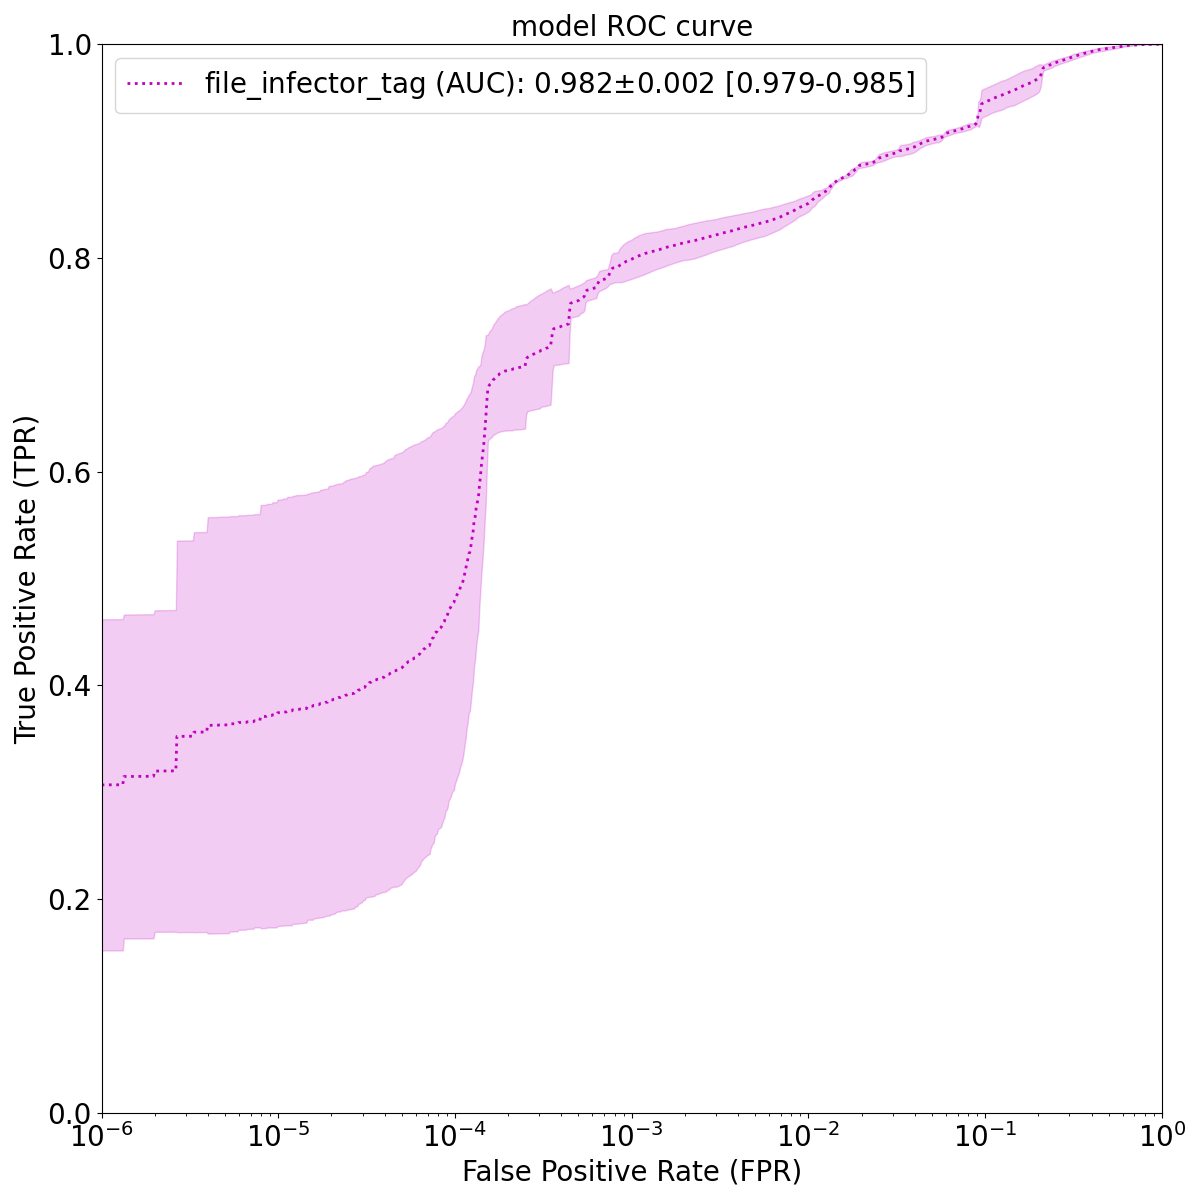
\includegraphics[width=0.6\textwidth]{./results/file_infector_tag_roc_aloha.png}
        \vspace*{-0.2cm}
        \caption[File-infector Tag prediction task ALOHA ROC curve]{ROC curve and AUC statistics of \textBF{ALOHA} model for the \textbf{File-infector Tag}. The line represents the \textit{mean} TPR at a given FPR, while the shaded region represents the \textit{standard deviation}. Statistics were computed over \textBF{2} training runs, each with random parameter initialization.}
        \label{fig:fileInfectorTagRocAloha}
    \end{figure}
}

\newcommand{\fileInfectorTagRocProposedMethod}{
    \begin{figure}[H]
        \vspace*{-0.5cm}
        \centering
        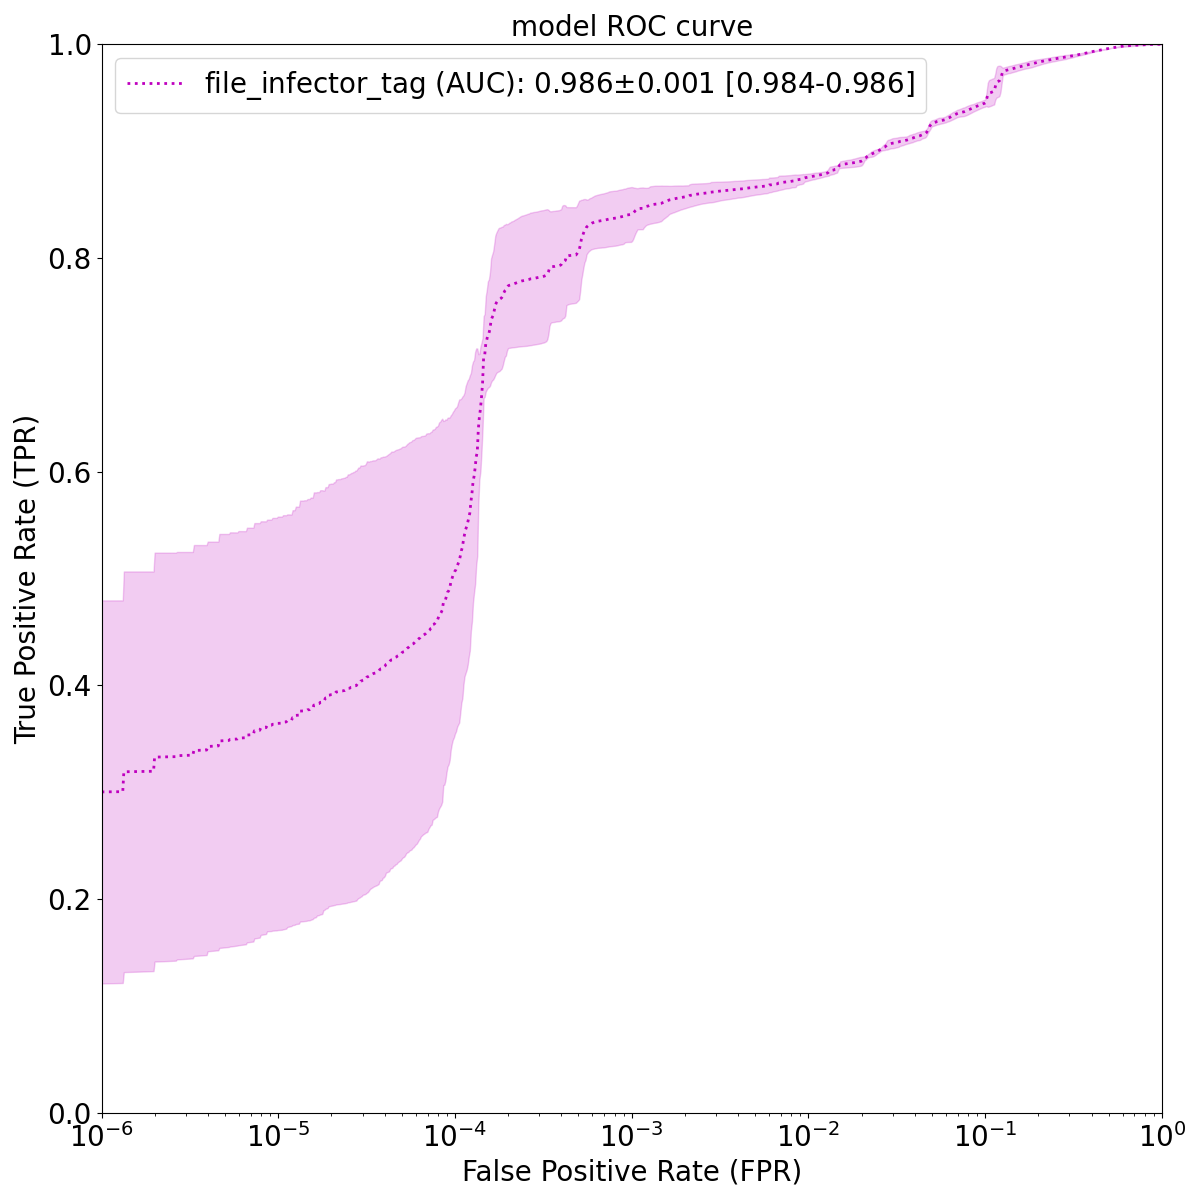
\includegraphics[width=0.6\textwidth]{./results/file_infector_tag_roc_proposedModel.png}
        \vspace*{-0.2cm}
        \caption[File-infector Tag prediction task Proposed Model ROC curve]{ROC curve and AUC statistics of \textBF{Proposed Model} for the \textbf{File-infector Tag}. The line represents the \textit{mean} TPR at a given FPR, while the shaded region represents the \textit{standard deviation}. Statistics were computed over \textBF{2} training runs, each with random parameter initialization.}
        \label{fig:fileInfectorTagRocProposedModel}
    \end{figure}
}
